\documentclass[aspectratio=169,11pt]{beamer}
\usetheme{Boadilla}
\usepackage[T1]{fontenc}
\usepackage{lmodern,booktabs,graphicx}
\definecolor{pyroblue}{RGB}{23,107,145}
\setbeamercolor{structure}{fg=pyroblue}
\setbeamercolor{title}{fg=pyroblue}
\setbeamercolor{frametitle}{fg=pyroblue,bg=black!3}
\setbeamertemplate{navigation symbols}{}
\setbeamertemplate{footline}{\hfill\scriptsize PYRO-KD \textbullet\ Revision 1.5 draft\hspace{1em}\insertframenumber/\inserttotalframenumber\hspace{1em}\vspace{2mm}}
\setbeamertemplate{itemize items}[circle]
\newcommand{\Acue}{A\textsubscript{cue}}
\newcommand{\source}[1]{\vfill{\tiny\color{gray}Evidence: #1}}
\title{Cue-Driven Keyframe Selection}
\subtitle{Audio description and video QA\newline Revision 1.5: local experiment evidence}
\author{PYRO-KD team\newline\small Human names and contribution attribution pending team confirmation}
\institute{NYU Computer Vision \textbullet\ Agent Track research project}
\date{Draft: 23 November 2026}
\begin{document}

\begin{frame}
\titlepage
\vspace{-4mm}
\begin{center}\small Formal core and QA aggregation remain pending.\newline Paid APIs and human labels are deferred; no human-quality claim.\end{center}
\end{frame}

\begin{frame}{Separate what matters from where narration fits}
\begin{columns}[T]
\column{.48\textwidth}
\begin{block}{Salience}
Visual novelty; speech cues;\newline non-speech events and acoustic change.
\end{block}
\begin{block}{Feasibility}
VAD gaps; two-second separation;\newline word cap $\lfloor3\Delta t\rfloor$.
\end{block}
\column{.48\textwidth}
\begin{block}{Frozen generation}
Four frames across two seconds.\newline P0 plain / P1 guidelines + three training exemplars.\newline Qwen2.5-VL; temperature zero.
\end{block}
\begin{alertblock}{Evaluate every transition}
Requested $\rightarrow$ selected $\rightarrow$ prepared $\rightarrow$ valid $\rightarrow$ rendered.
\end{alertblock}
\end{columns}
\source{Proposal Revision 1.5; frozen REFRAMED TOML and source 09abb6c.}
\end{frame}

\begin{frame}{The matrix and the scope actually evaluated}
\centering
\begin{tabular}{lll}
\toprule Benchmark & Frozen scope & Conditions \\
\midrule REFRAMED & 30 test clips; 10 dev & 5 selectors $\times$ 2 prompts \\
EgoSchema & 490 heldout; 10 pilot & U / V-local / V-memory \\
Long Video-MME & 12 videos; 36 questions & 10 conditions; 360 requests \\
\bottomrule
\end{tabular}
\vspace{5mm}
\begin{itemize}
\item Core plan: U, V, \Acue{}, AV, O $\times$ P0/P1 $\times$ local/API = 20 cells.
\item Ten local cells authorized; ten paid cells explicitly deferred (\$0 cap).
\item Proposal A is \Acue{}; O uses reference timestamps and is an upper bound.
\item EgoSchema has no distributed audio: visual-only diagnostic.
\end{itemize}
\source{Frozen split/config hashes; all 5,031 EgoSchema distributed videos probed; Cue2Narrate comparison unavailable.}
\end{frame}

\begin{frame}{Development losses remain visible}
\begin{columns}[c]
\column{.68\textwidth}
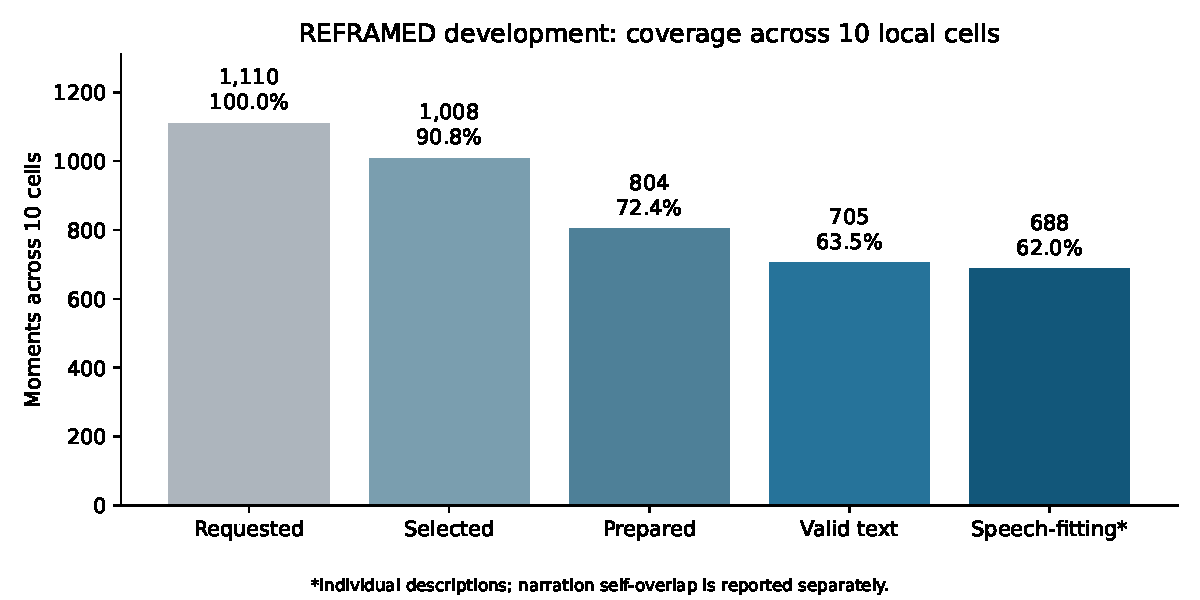
\includegraphics[width=\linewidth]{../results/reframed-dev-coverage.pdf}
\column{.30\textwidth}
\large 804 attempts\\[2mm]
\normalsize 705 valid captions\\
84 word-budget failures\\
15 token-limit failures\\[4mm]
\textbf{688 fit individually}\\
This does not exclude narration self-overlap.
\end{columns}
\source{Ten local development cells; actual Piper speech at 1.2$\times$; original 128-token pilot preserved.}
\end{frame}

\begin{frame}{Development evidence froze the formal protocol}
\begin{itemize}
\item Dev-only selector tuning; no heldout tuning or exemplar leakage.
\item Fifteen truncated dev cases probed at 512 tokens:\newline five finish at 128--139; ten continue looping.
\item Formal ceiling: 192 tokens, with failures retained rather than silently truncated into valid captions.
\item Long-QA resource smokes: 612 and 1,012 frames; resolution 224 px fixed before correctness scoring.
\item Formal AD source 09abb6c: 817 tests passed, 3 skipped, 5,974 subtests.
\end{itemize}
\begin{block}{Reuse after validation}
Pinned weights, compatible feature caches, immutable worker sources, and disjoint output ownership. No duplicate timeline-present ablation inference.
\end{block}
\source{Formal freeze record; token-ceiling diagnostic; real-data smoke logs; full formal-source pytest log.}
\end{frame}

\begin{frame}{Heldout selector agreement before caption generation}
\begin{columns}[T]
\column{.52\textwidth}
\centering
\begin{tabular}{lrr}
\toprule Selector & Selected / requested & F1 \\
\midrule U & 388/388 & .311 \\
V & 388/388 & .389 \\
\Acue{} & 384/388 & .505 \\
AV & 384/388 & .494 \\
O (oracle) & 366/388 & .839 \\
\bottomrule
\end{tabular}
\column{.44\textwidth}
\begin{itemize}
\item All 31 configurations cover all 30 clips.
\item Descriptive clip-mean temporal F1 at$\pm2$s.
\item Selection agreement is not caption correctness.
\item Audio-event human validation remains absent.
\end{itemize}
\end{columns}
\vspace{4mm}
\small Selector ablation family: 16 movie-clustered contrasts across 10 movies; all Holm-adjusted $p=1.0$. Family declared after descriptive results; not preregistered. No validated ablation winner.
\source{reframed-selectors and reframed-selector-ablations exports; no settings changed after these heldout results.}
\end{frame}

\begin{frame}{Formal audio context: coverage changes with the condition}
\centering
\begin{tabular}{lrrr}
\toprule \Acue{}/P0 context & Valid / 384 & Temporal F1 & TTS fit / rendered \\
\midrule None (Qwen) & 349 & .469 & 345/349 \\
Text timeline (Qwen) & 372 & .521 & 370/372 \\
Native audio (Omni) & 326 & .465 & 324/326 \\
\bottomrule
\end{tabular}
\vspace{5mm}
\begin{itemize}
\item Same 384 prepared moments; selector chosen on development data.
\item All 30 test clips remain in temporal denominators.
\item Native audio changes the model as well as modality.
\item Conditional text similarity and individual speech fit do not establish human preference or combined playback quality.
\end{itemize}
\source{Verified formal ablation 5 exports; core timeline predictions reused; no significance claim on this slide.}
\end{frame}

\begin{frame}{A valid caption can still fail during playback}
\begin{columns}[T]
\column{.48\textwidth}
\begin{block}{Word-compliant, but too long in seconds}
A six-word dev caption meets its six-word cap.\\[2mm]
Rendered at 1.2$\times$:2.525s.\newline Available machine speech-free interval:2.200s.\\[2mm]
\textbf{Speech collision: 0.325 s.}
\end{block}
\column{.48\textwidth}
\begin{block}{Individually fitting, jointly overlapping}
Caption 1:[27.5,34.429]s\newline Caption 2:[34.0,36.830]s\\[2mm]
Both avoid machine-labeled original speech.\\[2mm]
\textbf{AD--AD overlap: 0.429 s.}
\end{block}
\end{columns}
\small Formal timeline ablation totals 729.971 s of excess overlapping narration, despite 370/372 individual fits. A future narration scheduler is a separate method.
\source{Development qualitative review with IDs, frame/WAV hashes and actual overlap rows; agent inspection, not human labels.}
\end{frame}

\begin{frame}{Long-video QA has a constrained realized budget}
\begin{columns}[T]
\column{.48\textwidth}
\begin{block}{Requested budget}
2,314 moments\newline 4 frames per moment\newline 9,256 frames for U
\end{block}
\column{.48\textwidth}
\begin{block}{Flat \Acue{} realized budget}
1,497 moments\newline 5,988 frames\newline Safe-gap capacity limits selection
\end{block}
\end{columns}
\begin{itemize}
\item All 12 audio/source gates passed; shortfalls are not missing media.
\item Video 604: 153 requested moments, capacity 14; machine VAD marks 97.4\% speech.
\item A/AV results are \textbf{constrained-budget diagnostics}, not equal-realized-frame-budget evidence.
\item Added missing A/AV timeline-off controls before any correctness scoring; their frame lists exactly match timeline-on.
\end{itemize}
\source{Long selection-capacity audit; frozen ten-condition/13 contrast QA family; no arbitrary filling or test tuning.}
\end{frame}

\begin{frame}{Final core and QA results: pending verified aggregation}
\begin{alertblock}{Do not substitute development numbers}
Fill the ten local core rows and the QA results only after prediction coverage, text metrics, actual speech checks, and paired exports finish.
\end{alertblock}
\begin{itemize}
\item Core: 3,398 prepared requests; retain all 30clips, missing/failed IDs, and zero-output videos.
\item EgoSchema: 490 questions per condition; failures count incorrect.
\item Long QA: 36 questions per condition across 12 video clusters.
\item Paired bootstrap intervals, Wilcoxon tests, Holm within declared families.
\item Report all deferred paid rows and unvalidated human requirements.
\end{itemize}
\source{Frozen protocols and comparison families; this slide intentionally contains no pending-result estimates.}
\end{frame}

\begin{frame}{Agent verification: failures that changed the workflow}
\begin{tabular}{p{.42\textwidth}p{.50\textwidth}}
\toprule Failure & Verification / repair \\
\midrule Stale output reuse & Source/config/split/exemplar identity guards \\
Missing videos omitted & Expected membership and zero-output coverage \\
Budget errors looked compliant & Complete-decode denominator; truncation unknown \\
Truncated JSONL resume & Backup + final-fragment recovery; interior corruption fails \\
False cache failure & Reload published metadata; reuse verified features \\
Wrong formal TTS cache & Correct external watcher; reuse existing renders \\
\bottomrule
\end{tabular}
\vspace{4mm}
\small Tests, real-data smokes, raw-ID accounting, hashes, and measured speech checks complement each other. Scheduler success alone is not scientific validation.
\source{Agent Log appendix and chronological English log; human contributions require team confirmation.}
\end{frame}

\begin{frame}{What the evidence supports—and what remains open}
\begin{itemize}
\item Cue-driven selectors have higher descriptive placement means than U on the frozen subset; selection alone does not guarantee usable narration.
\item The audio-context ablation exposes coverage and playback tradeoffs.
\item Final core/QA conclusions await completed verification.
\item No Cue2Narrate baseline claim, equal-realized-budget long-audio claim, or human-quality claim.
\end{itemize}
\begin{block}{Remaining requirements}
Paid-model/rubric authorization; human detector labels; blinded peer ratings; confirmed human contributions and team code walkthrough.
\end{block}
\small Reproduce: \texttt{docs/RESULTS\_REPRODUCTION.md}\newline Code and artifacts: \url{https://github.com/Yvonne-Yu217/PYRO-KD}
\end{frame}
\end{document}
